%% This LaTeX-file was created by Maarten van Leunen

%% Do not edit this file unless you know what you are doing.
\documentclass{article}
\usepackage[T1]{fontenc}
\usepackage{graphics}

\begin{document}
\author{Maarten van Leunen}
\title{MMUD\\Maarten's Mud}
\maketitle
\tableofcontents
\listoffigures
\listoftables
\newpage

\subsection{Legal Notice}
\begin{verbatim}
/*-------------------------------------------------------------------------
Maarten's Mud, WWW-based MUD using MYSQL
Copyright (C) 1998  Maarten van Leunen

This program is free software; you can redistribute it and/or
modify it under the terms of the GNU General Public License
as published by the Free Software Foundation; either version 2
of the License, or (at your option) any later version.

This program is distributed in the hope that it will be useful,
but WITHOUT ANY WARRANTY; without even the implied warranty of
MERCHANTABILITY or FITNESS FOR A PARTICULAR PURPOSE.  See the
GNU General Public License for more details.

You should have received a copy of the GNU General Public License
along with this program; if not, write to the Free Software
Foundation, Inc., 59 Temple Place - Suite 330, Boston, MA  02111-1307, USA.

Maarten van Leunen
Driek van Erpstraat 9
5341 AK Oss
Nederland
Europe
maartenl@il.fontys.nl
-------------------------------------------------------------------------*/
\end{verbatim}

\subsection{Acknowledgements}
I'd like to thank all the people that have been a support to me for so long
over the years. The Land of Karchan has had it's ups and downs over the
years as some of you might know, but now the source code is available with
which the Land of Karchan was created, and everyone who is familiar with
Linux can join and make their own.

I'd like to thank some of the people especially who helped me to build the
source code and were actually invaluable to me by giving practical advice
concerning source code. In no particular order they are Edwin Mons (edwinm), Mathijs
Brands (shrike), Joop Carels (zombie), Sven Berkens (sven), George Schroder
(frodpo). I also like to thank Steffan O'Sulivan for his excellent booklet
about "FUDGE" which helped me out a lot. I also like to thank Samual Jackson
Games for providing "GURPS" from which I learned a lot. I also like to thank the people
without whom this might never have come off the ground, the people of the
Open Source Movement, who have liberally provided me with the tools I needed
to make the Land of Karchan a reality.

\subsection{About the Author}
Well, let me introduce myself. I am Maarten van Leunen, currently living in
Oss, the Netherlands, Europe. Basically, when I entered College I for the
first time got into contact with Unix like Operating Systems, not by
studying, but by joining in the local InternetUsersAssociation Interlink. I aquired lots
of experience and knowledge there.

The first step towards creating a mud, ofcourse, is playing one. I happened
to frequent some time on Angalon, however, in time one has ambitions to
create one's own mud. At the same time, I was working on my first Homepage,
my first Guestbook. And when surfing I found out about a Mud consisting
entirely of links on the World Wide Web. I thought the idea was nifty, and
tried my hand at it. Then the idea crossed my mind to attempt to integrate
the experience I got from creating my Guestbook and my Homepage with the
experience of creating a Linked Mud. Apparently it has come this far, and
there is no end in sight just yet.

\newpage
\section{Installation}
\subsection{Root Priviledges}
It's a really bad idea to have this mud running under Root privileges. It's
a security issue. In stead, I suggest that you create a new user on your
server called "mmud". (or something else, in which case you need to make
some changes to the source code)

It's a mistake to run any kind of CGIbinary which is accessible from the
outside setuid root. It gives crackers the opportunity to enter your system
using this CGI.

\vspace{0.3cm}
{\par\centering \resizebox*{1\textwidth}{!}{\rotatebox{270}{\includegraphics{sourcecode.ps}}} \par}
\vspace{0.3cm}

\newpage
\section{Playing the game}
\subsection{Character Defaults}
The five main attributes of your character are:
\begin{itemize}
\item Strength
\newline
You can carry more if you are stronger.
\item Intelligence (mental skills)
\newline

\item Dexterity (physical skills)
\newline
Dexterity is a measurement of agility and coordination. Basically it says
how clumsy you are (or not).
\item Constitution
\item Wisdom
\end{itemize}

The five main attributes of an Elf are:
\begin{itemize}
\item Strength 2
\item Intelligence (mental skills) 2
\item Dexterity (physical skills) 1
\item Constitution 2
\item Wisdom 2
\end{itemize}

The five main attributes of an Dwarf are:
\begin{itemize}
\item Strength 2
\item Intelligence (mental skills) 1
\item Dexterity (physical skills) 2
\item Constitution 2
\item Wisdom 0
\end{itemize}

The five main attributes of a standard Human are:
\begin{itemize}
\item Strength 1
\item Intelligence (mental skills) 1
\item Dexterity (physical skills) 1
\item Constitution 1
\item Wisdom 1
\end{itemize}

The five main attributes of a Faery are:
\begin{itemize}
\item Strength 0
\item Intelligence (mental skills) 2
\item Dexterity (physical skills) 1
\item Constitution 1
\item Wisdom 2
\end{itemize}

\subsection{Weight and Encumberance}
The amount of stuff you are carrying and the amount of strength you have
determines how much of your movement is spent on each move.

\begin{itemize}
\item weight < 500 + 50*Strength => no penalty
\item weight < 1000 + 50*Strength => move penalty of 10
\item weight < 1500 + 50*Strength => move penalty of 20
\item weight < 2000 + 50*Strength => move penalty of 30
\item weight < 2500 + 50*Strength => move penalty of 40
\item weight < 3000 + 50*Strength => move penalty of 50
\item weight >= 3000 + 50*Strength => UNABLE TO MOVE
\end{itemize}

So, to summarize. If you carry too much, you cannot move. The more you
carry, the more you get exhausted (i.e. lose movement points). Once you are
exhausted you cannot move. You recover over time, but it takes some time to
recover fully.
The stronger you are, the more you can carry and the less movement points it
takes for you to move.

\subsection{Skills}

Skills are defined as Items in this game. It is for example possible to own
an item called "\emph{Swordplay}". The Skilllevel inherent to the item is
stored in "skillevel". The skilllevel is a minimum of 0 and a maximum of 18.
If you have not "learned" the skill, the item does not exist.

A skill is relative to one of the five main attributes of your character.
The five main attributes of your character are:
\begin{itemize}
\item Strength
\item Intelligence (mental skills)
\item Dexterity (physical skills)
\item Constitution
\item Wisdom
\end{itemize}

If your skill level reaches beyond a certain level, as to be successfull
without really trying, the skill (in case for example with magic skills)
must be removed or automatically changed onto a higher skill. For example a
magic skill cast "\emph{burning candle}" should automatically revert to the
beginning level of "\emph{small fireball}" possibly converging all the way
to "\emph{firestorm}".

\subsection{Success Rolls}
A "success roll" is a die roll made when you need to "test" one of your
skills or abilities.. You roll against something, for instance an ability with an
Skill. This game predominately uses rolls against skills in order to see if
they will succeed or not. If your roll is less than or equal to the skill or
ability you are testing, you succeeded. Otherwise, you failed. Thus, the
higher the stat you are rolling against, the easier it is to make the roll.

For instance, if you have a skill "Swordplay", with "skillevel" 10, you roll
three dice. If the number of eyes is below or equal to 10, you succeed
otherwise you fail. A roll of 17 or 18 is an automatic and possibly
spectacular failure to practise the skill.

Ofcourse, you only need a "successroll" if you have a sword in your hand and
a skill "Swordplay". Otherwise the successroll is irrelevant. In the case
where a person is not holding anything in his hands, success will be
dependent on your skill at "unarmed combat".

\paragraph{Critical Success and Critical Failure}
There is such a thing as critical success if you (the computer) rolls the
dice and the outcome is either 3 or 4. This constitutes a critical success
with exceptional results if possible. A critical success has no chance of a
defense, all your hits strike home at your opponent.

There is such a thing as a critical failure if you (the computer) rolls the
dice and the outcome is 18. This constitutes a critical failure with
inordinately bad results.

\subsection{Reaction Rolls}
Not implemented yet. Perhaps not necessary.

\subsection{Defense Rolls}
Your foes defence equals \emph{passive} and \emph{active} defenses.
Passive defense is \emph{armour} and \emph{shields}. Active defense are skills
like \emph{dodge}, \emph{block}, \emph{parry}.

If the defense is successfull, no damage is done, and no damage roll is
executed.

\subsection{Damage Rolls}
A damage rolls is done in order to see how much damage you to do to your
opponent. A few things can effect the amount of damage you do, for instance:

\begin{itemize}
\item armour
\item weapon
\end{itemize}

\subsection{Learning and Improving Your Character}
Improving your character is done by learning a skill first, and then
improving upon it.

You can learn Skills by using the "\emph{practises}" which you have gained
when levelling. Every time you level, you gain 1 practise. That can be spent
on learning a certain skill.

You can improve Skills by using the "\emph{practises}" which you have gained
when levelling. Every time you level, you gain 1 practise. That can be spent
on a certain skill to up it one point.

You can improve your standard attributes by using the "\emph{training}"
points you got when you levelled. It can be used to gain a point in one of
the 5 attributes:
\begin{itemize}
\item Strength
\item Intelligence (mental skills)
\item Dexterity (physical skills)
\item Constitution
\item Wisdom
\end{itemize}

\section{Special Rooms}
\subsection{Moneychanger Office}
The money changers office has a special meaning. It can translate your coins
to another currency value (gold, copper, or silver) and you can open and
close and mutate an account there. For the most part it works just like a
bank.

To explain how the translation of coins work, we have to realize that, if we
use the copper coins as common denominator, the gold coins are worth 100
copper coins and the silver coins are worth 10 copper coins. A simple   
calculation does suffice to make converting values possible.

To explain how the bank principle works. If you open an account three items
in the tmp\_itemtable are created. Item 36 is copper coins, search=you,
room=-1 and the rest is empty. The same goes for Item 37 (silver) and item
38 (gold). The "amount" field takes care of the amount of gold silver or  
copper coins you have in your account. Withdraw and deposit simply mutate 
the gold, silver, copper fields in your character sheet as well as the    
amount in the different tmp\_itemtable items.

\section{Combat}
\subsection{Who is fighting who?}
The only way to determine wether or not a person is fighting another person
and wether or not it is necessary to compute hits and start whacking each
other depends on a number of settings, written down here.

First of all, we will proceed from the assumption that character X is
fighting character Y. We now have to determine if this fight is actually
legal. The following constraints apply:
\begin{itemize}
\item ExistUser(X) == true (User X is active in the game)
\item ExistUser(Y) == true (User Y is active in the game)
\item X.sleep == false (User X is not asleep)
\item Y.sleep == false (User Y is not asleep)
\item X.room == Y.room (User X and Y are in the same room together)
\item Y.god != 2 (User Y is not a non-killable bot)
\item X.fightable == true (User X may fight people)
\item Y.fightable == true (User Y may be fought against)
\item X.fightingwho == Y.name (User X is definitely trying to fight User Y)
\end{itemize}
This part translates into the following SQL statement that has been used in
the "rolls.c" file:
\begin{itemize}
\item select X.*, Y.* from tmp\_usertable as X, tmp\_usertable as Y where
X.fightingwho = Y.name and
X.sleep = 0 and
Y.sleep = 0 and
X.room = Y.room and
Y.god != 2 and
X.fightable = 1 and
Y.fightable = 1;
\end{itemize}

\vspace{0.3cm}
{\par\centering
\resizebox*{1\textwidth}{!}{\rotatebox{270}{\includegraphics{compute_hit.ps}}} \par}
\vspace{0.3cm}

\subsection{Defense}
Every item that you use in combat has both a passive defense and an active
defense. The passive defense is the defence the item gives you without you
having to do anything (for example, making you hard to hit), the active
defense is when you actively do something with the item (like parry).

\begin{verbatim}
Combat Mathmatics
-----------------
						Easy	Most	Hard	VH
Terrible		-2		-1		0			1
Poor				-1		0			1			2
Mediocre		0			1			2			3
Fair				1			2			3			4
Good				2			3			4			5
Great				3			4			5			6
Superb			4			5			6			7

Terrible	-3
Poor			-2
Mediocre	-1
Fair			0
Good			1
Great			2
Superb		3

- Three die roll
- Select median (the middle rolled value)
	Mediocre	Good	Great		=>	Good
	Poor	Great	Great				=>	Great
- decides which trait to use
- modifier from -3,0,+3, depending on armour, wounds, special abilities
etcetera, modifier, so {(current skill of player + modifier) = total}
-

HURT = > -1 to all actions

Critical Result:
When throwing dice really badly, one could make the following critical
table;
2. blinded for next combat round
3. fall down
4. off balance
5. lose/drop weapon
6. weapon breaks -> gone forever.


Compute Hit

Difficulty

Character has skill-level
Object has skill-level
If char.skilllevel>=obj.skillevel => succeed
if char.skillevel<obj.skilllevel => rolldice
"appraise" command

Magic
-----

- niet cumulatief

Melee:	any combat that involves striking the opponent with a fist or
hand-held weapon. Any attack from further away is a Ranged attack.
Alternating combat turns.

Combat Round: an indeterminate length of time set by the GM - around three
seconds seems reasonable to some people, while that seems grossly short or
absurdly long to others. A given GM's combat round may vary in length,
depending on the situation. Generally, when each character involved has made
an action, a given round is over.

Offensive damage factors: those which contribute to damaging an opponent
Strength (is using a Strength-driven weapon) Scale and deadliness of
weapon.

Defensive damage factors: those which contribute to reducting the severity
of a received blow: Scale, armor, and possibly Damage Capacity.

Total damage factor (or simply damage factor): the attacker's offensive
damage factor minus the defender's defensive damage factor.

Damage:

- weapon-type
-

relative degree 0 :
- nobody gets hurt
- blow on shield

- Opposed action
- Unopposed action

- Shield
- Dodge
- Parry

- All-out attack
- All-out defense

- bad footing, lower elevation, light in his eyes, kneeling

\end{verbatim}



\subsection{Illness, injury and Fatigue}

\subsection{Magic}

\section{Maps}
Maps will be created using Gimp. The text contained on the map is "times" and the size = 12.

\newpage
\section{Appendix A  - Table Description}

\subparagraph{action}table containing descriptions of special actions that
are allowed in some rooms
\subparagraph{answers}table containing all the different answers by bots on
questions asked
\subparagraph{bantable}table containing who is banned, why, by whom, for how
long at which time, etc.
\subparagraph{bogus\_itemtable}this is a very strange table that is currently being used as a temporary table for the cleaning up of corpses in the game. (see also the script mysql_healing)
\subparagraph{bottable}table containing the bots, gets copied periodically
to the tmp\_usertable by a crontab entry in order to add bots that people
have fought against and killed
\subparagraph{bugreportlist}list of bugs still to be solved
\subparagraph{depalias}special commands for the deputies to use
\subparagraph{help}help on commands
\subparagraph{items}item definitions
\subparagraph{itemtable}all items
\subparagraph{logonmessage}contains the logonmessage when you enter the game
\subparagraph{mailtable}all mail
\subparagraph{olditem}archived/deleted items
\subparagraph{oldmail}archived/deleted mail
\subparagraph{olduser}archived/deleted users
\subparagraph{respawningitemtable}items that need to reappear after a
certain time
\subparagraph{rooms}description of all rooms, along with exits
\subparagraph{sillynamestable}contains silly names/bad language in order to
root out bad logonids in entering the game
\subparagraph{skills}skill definitions
\subparagraph{skilltable}all skills
\subparagraph{tmp\_itemtable}items during gameplay
\subparagraph{tmp\_mailtable}mail during gameplay
\subparagraph{tmp\_usertable}users during gameplay
\subparagraph{todo}todo list
\subparagraph{unbantable}people that are allowed to login despite the fact
that their site/domain is banned
\subparagraph{usertable}all users

\section{Appendix B  - Field Description}

\paragraph{usertable}
\subparagraph{name}the uniquely identifying name of a player character
\subparagraph{address}the ip address or host name from where the character
is being controlled
\subparagraph{password}
\subparagraph{title}
\subparagraph{realname}
\subparagraph{email}
\subparagraph{race}
\subparagraph{sex}
\subparagraph{age}
\subparagraph{length}
\subparagraph{width}
\subparagraph{complexion}
\subparagraph{eyes}
\subparagraph{face}
\subparagraph{hair}
\subparagraph{beard}
\subparagraph{arm}
\subparagraph{leg}
\subparagraph{gold}
\subparagraph{silver}
\subparagraph{copper}
\subparagraph{room}
\subparagraph{lokwhimpy}
\subparagraph{experience}
\subparagraph{fightingwho}
\subparagraph{sleep }
\subparagraph{punishment}
\subparagraph{fightable }
\subparagraph{vitals}
\subparagraph{fysically }
\subparagraph{mentally}
\subparagraph{drinkstats}
\subparagraph{eatstats}
\subparagraph{active}
\subparagraph{lastlogin datetime}
\subparagraph{birth datetime}
\subparagraph{god }
\subparagraph{guild}
\subparagraph{strength}
\subparagraph{intelligence}
\subparagraph{dexterity }
\subparagraph{constitution}
\subparagraph{wisdom}
\subparagraph{practises }
\subparagraph{training}
\subparagraph{bandage }
\subparagraph{alignment }
\subparagraph{manastats }
\subparagraph{movementstats }
\subparagraph{maxmana }
\subparagraph{maxmove }
\subparagraph{maxvital}
\subparagraph{cgiServerSoftware}
\subparagraph{cgiServerName}
\subparagraph{cgiGatewayInterface}
\subparagraph{cgiServerProtocol}
\subparagraph{cgiServerPort}
\subparagraph{cgiRequestMethod}
\subparagraph{cgiPathInfo}
\subparagraph{cgiPathTranslated}
\subparagraph{cgiScriptName}
\subparagraph{cgiRemoteHost}
\subparagraph{cgiRemoteAddr}
\subparagraph{cgiAuthType}
\subparagraph{cgiRemoteUser}
\subparagraph{cgiRemoteIdent}
\subparagraph{cgiContentType}
\subparagraph{cgiAccept}
\subparagraph{cgiUserAgent}
\subparagraph{jumpmanaint}
\subparagraph{jumpmoveint}
\subparagraph{jumpvital}

\paragraph{skills}
\subparagraph{id}the id number of the skill (connection with skilltable
\subparagraph{name}the name of the skill, for example, \emph{Swordplay}
\subparagraph{inlevel}level needed at which the skill becomes available and can be learned
\subparagraph{outlevel}level at which the skill becomes to basic and is erased from memory
\subparagraph{manacost}the amount of mana it costs to use the skill or magic spell
\subparagraph{begineffect}description
\subparagraph{endeffect}description
\subparagraph{modifiername}1=Strength,2=Dexterity,3=Intelligence,4=Wisdom,
5=Constitution,...
\subparagraph{difficulty}1=easy,2=average,3=hard,4=veryhard
\subparagraph{type}1=normal skill, 2=fight skill, 3=magic skill, 4=cleric skill

\paragraph{skilltable}
\subparagraph{id}reference to skills-table
\subparagraph{forwhom}reference to tmpusertable/usertable
\subparagraph{skilllevel}

\paragraph{items}
\subparagraph{id}
id number of the item
\subparagraph{wieldable}wether or not the item can be wielded in hand. 0=not
wieldable, 1=wieldable right hand, 2=wieldable left hand, 3=wieldable both
hands
\subparagraph{wearable}wether or not the item can be worn on body. 0=not
wearable, 1=wearable on lefthand, 2=wearable on right hand, 3=wearable on
both hands, 4=wearable on head, 7=wearable on neck, 8=wearable on head,
9=wearable on body, 10=wearable on legs, 11=wearable on feet

\paragraph{tmp\_itemtable}
This table, compared to the "itemtable" does not have any differences apart
from the fact that this table only contains the currently used items in the
game. The "itemtable" contains the items that are saved upon quitting the
game and are retrieved upon (re)entering the game.
\subparagraph{id}
id number of the item, foreign key to "items"
\subparagraph{wearing}
where on body the item is worn. An empty string means that it isn't worn at
all. Possiblities are "lefthand", "righthand", "head", "neck", "head",
"body", "legs", "feet"
\subparagraph{wielding}
on which hand the item is wielded. An empty field meaning that it isn't
wielded at all. Possibilities are 1 (right hand) and 2 (left hand)

\newpage

\section{Appendix C - Database Structure}

\vspace{0.3cm}
{\par\centering
\resizebox*{1\textwidth}{!}{\rotatebox{270}{\includegraphics{database.ps}}} \par}
\vspace{0.3cm}

\section{Appendix D - Rolls Analysis}

First "main" started.

"main" starts "StartSQL".

"StartSQL" uses "checkBestHand" to determine which hand (along with which
item) to use during combat, so, depending on outcome of "checkBestHand"
"StartSQL" determines wether to choose "right" or "left". Two choices in the
If-then statement.

"checkBestHand" provides you with wether the "right" hand or the "left" hand
is the best. There are three possible scenarios, neither hand contains an
item (returns right hand), one hand contains item (returns hand that
contains item) and both hands contain items (returns hand with best shot).
In the last case, "checkBestHand" uses "checkWeaponSkill" to determine which
one of the two hands has the better skill in item carrying.

After that, the "AttackRoll" determines wether or not the attempt to strike
your opponent is successfull. Either it is successfull (you hit your
opponent) or it isn't successfull (you missed). However, there is the
possiblity of a FANTASTIC success or a FATAL failure, which is just an
extreme version of the previously described process.

After the Attackroll has been successfull, it is necessary to compute a
"DefenseRoll". If the defense of your opponent is successfull, you succeed
in hitting him but do not do any damage. 

If your opponent fails to defend himself, you have to have a "DamageRoll".
The DamageRoll determines how much of your hit has been transferred to
actual damagepoints on the part of your opponent.

\vspace{0.3cm}
{\par\centering
\resizebox*{1\textwidth}{!}{\rotatebox{270}{\includegraphics{rolls2.ps}}} \par}
\vspace{0.3cm}

\newpage
\section{Appendix E - Examples of Skills}

Unarmed Combat
\newline
Dodge
\newline
Parry (with most weapons)
\newline
Block (only with shield)
\newline
Combat Reflexes
\newline
Thrusting
\newline
Swinging
\newline
Throwing
\newline
Impaling

... your text goes here ...
\end{document}
